\documentclass[border=6pt]{standalone}
\usepackage[T1]{fontenc}
\usepackage[utf8]{inputenc}
\usepackage[scaled=0.98]{helvet}
\renewcommand{\familydefault}{\sfdefault}
\usepackage{amsmath}
\usepackage{graphicx}
\graphicspath{{../../../../../../exercises_lecturenotes/lecture_notes/kurs100_lektionsnoter/}}
\usepackage{tikz}
\usepackage{pgfplots}
\pgfplotsset{compat=1.18}
\usetikzlibrary{arrows.meta, decorations.pathreplacing, calc, positioning, fit, backgrounds, shapes.geometric}
\usepgfplotslibrary{groupplots,fillbetween}
\definecolor{scanpink}{HTML}{E5006D}
\definecolor{scanteal}{HTML}{00A6A6}
\definecolor{scannavy}{HTML}{243746}
\definecolor{scanlightgray}{HTML}{F1F2F3}
\begin{document}
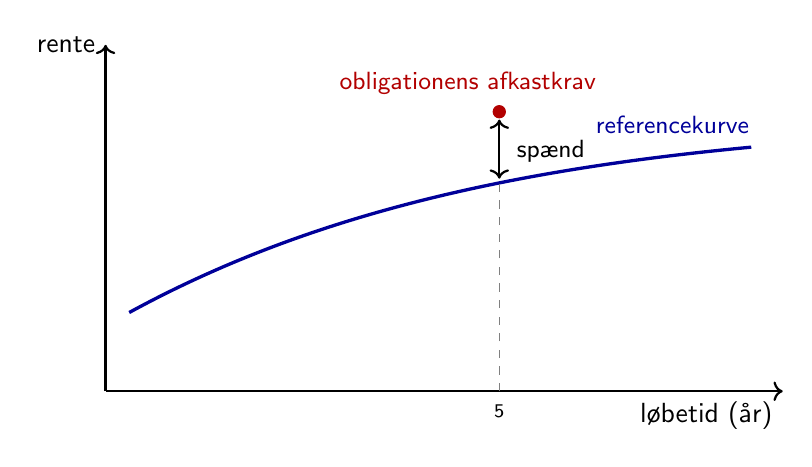
\begin{tikzpicture}[scale=1.0]
  % akser
  \draw[->, thick] (0,0) -- (8.6,0) node[below left] {løbetid (år)};
  \draw[->, thick] (0,0) -- (0,4.4) node[left] {rente};
  % referencekurve
  \draw[very thick, blue!60!black] (0.3,1.0) .. controls (2.5,2.2) and (5,2.8) .. (8.2,3.1);
  \node[blue!60!black, font=\small, above] at (7.2,3.15) {referencekurve};
  % obligationens afkastkrav
  \filldraw[red!70!black] (5,3.55) circle (2.2pt);
  \node[red!70!black, font=\small, above] at (4.6,3.65) {obligationens afkastkrav};
  % spænd
  \draw[<->, thick] (5,2.70) -- (5,3.45);
  \node[font=\small, right] at (5.1,3.05) {spænd};
  % hjælpelinje
  \draw[dashed, gray] (5,0) -- (5,2.70);
  \node[font=\scriptsize, below] at (5,-0.05) {5};
\end{tikzpicture}
\end{document}
